\newpage
\subsection{correct}
This section lists all the corrections that can be performed. It is logged in the datafile whether a certain correction has already been performed, in the \emph{exp\_name.h.det\_name.corr\_log} field.
First of all, the coordanite system used in this software is defined in Figure \ref{coor_sys}.

\begin{figure}
  \centering
  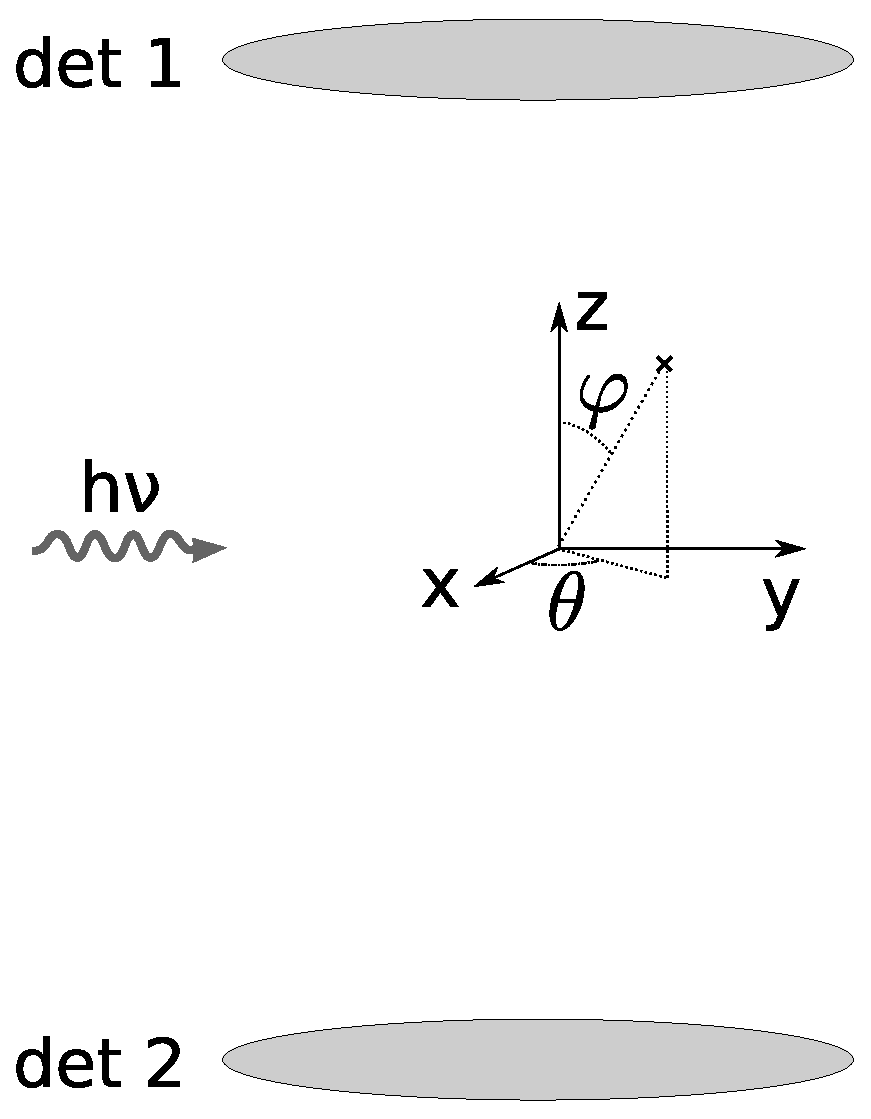
\includegraphics[width=0.5\textwidth]{Graphics/coordinate_system.eps}
  \captionof{figure}{Definition of coordinate system used in this Software. The x-axis aligns with the polarization and the molecular beam, the Y-direction aligns with the photon beam, and Z aligns with the detector axis.}
\label{coor_sys}
\end{figure}

\subsubsection{detection image translation}

\begin{figure}
\centering
\begin{minipage}{.5\textwidth}
  \centering
  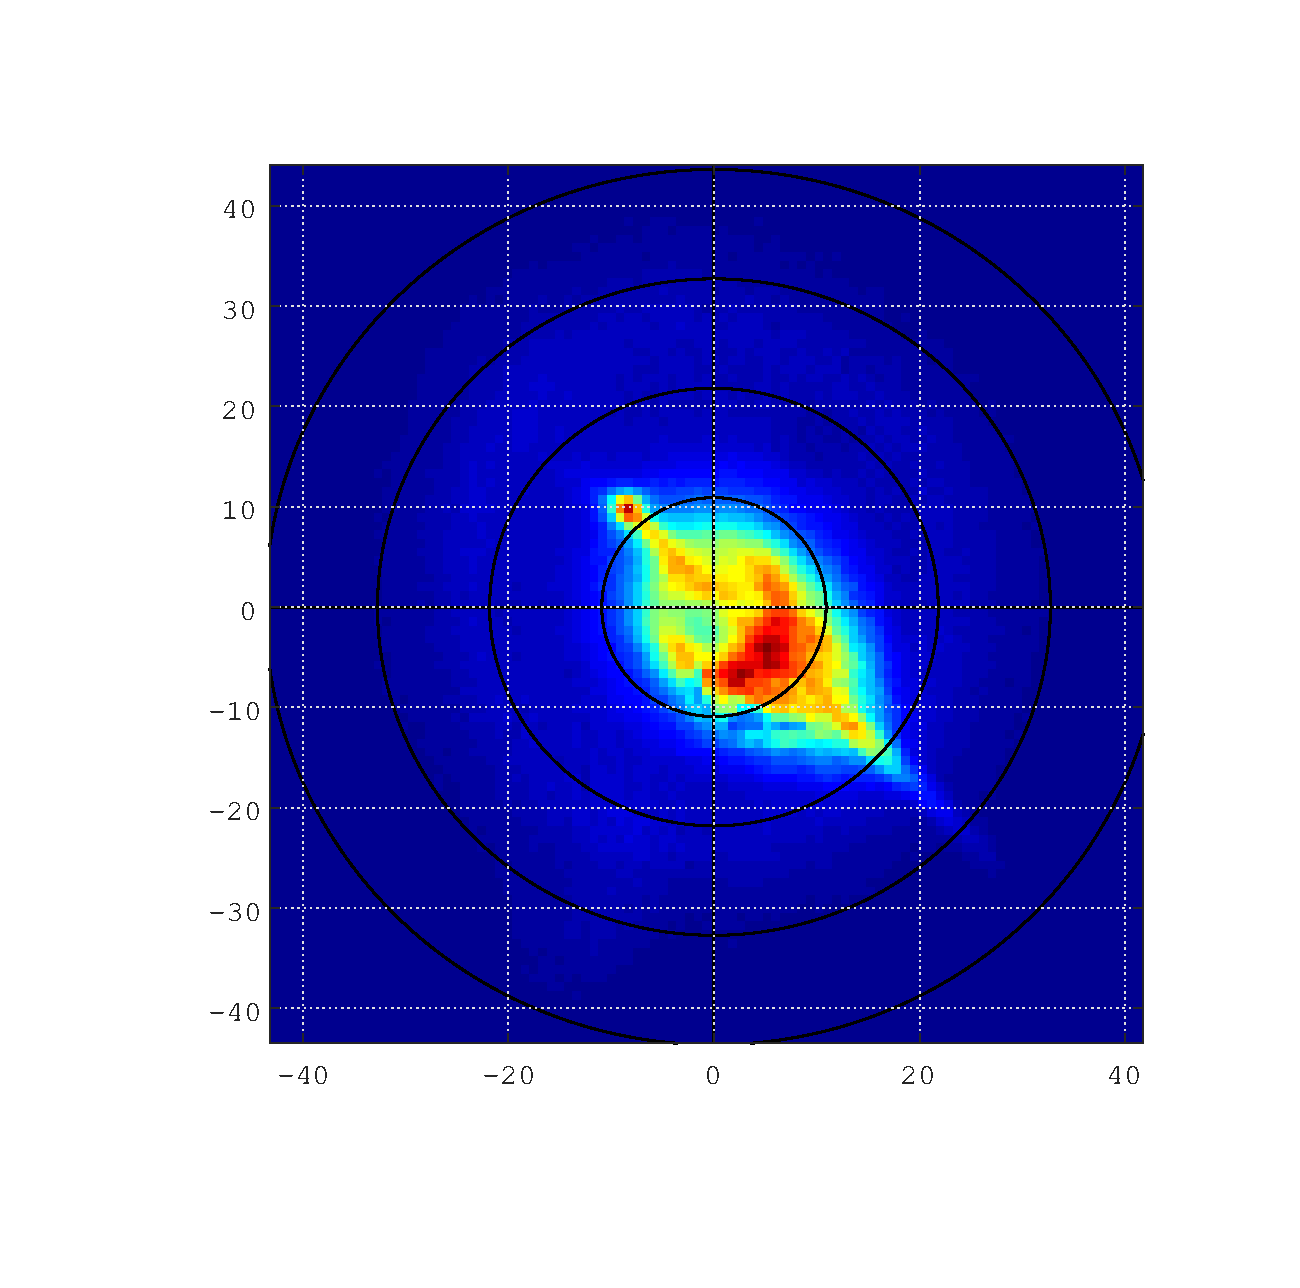
\includegraphics[width=1\textwidth]{Graphics/centre_calibration_before.eps}
  \captionof{figure}{Detector image of all hits before centring}
\label{centre_calibration_before}
\end{minipage}%
\begin{minipage}{.5\textwidth}
  \centering
  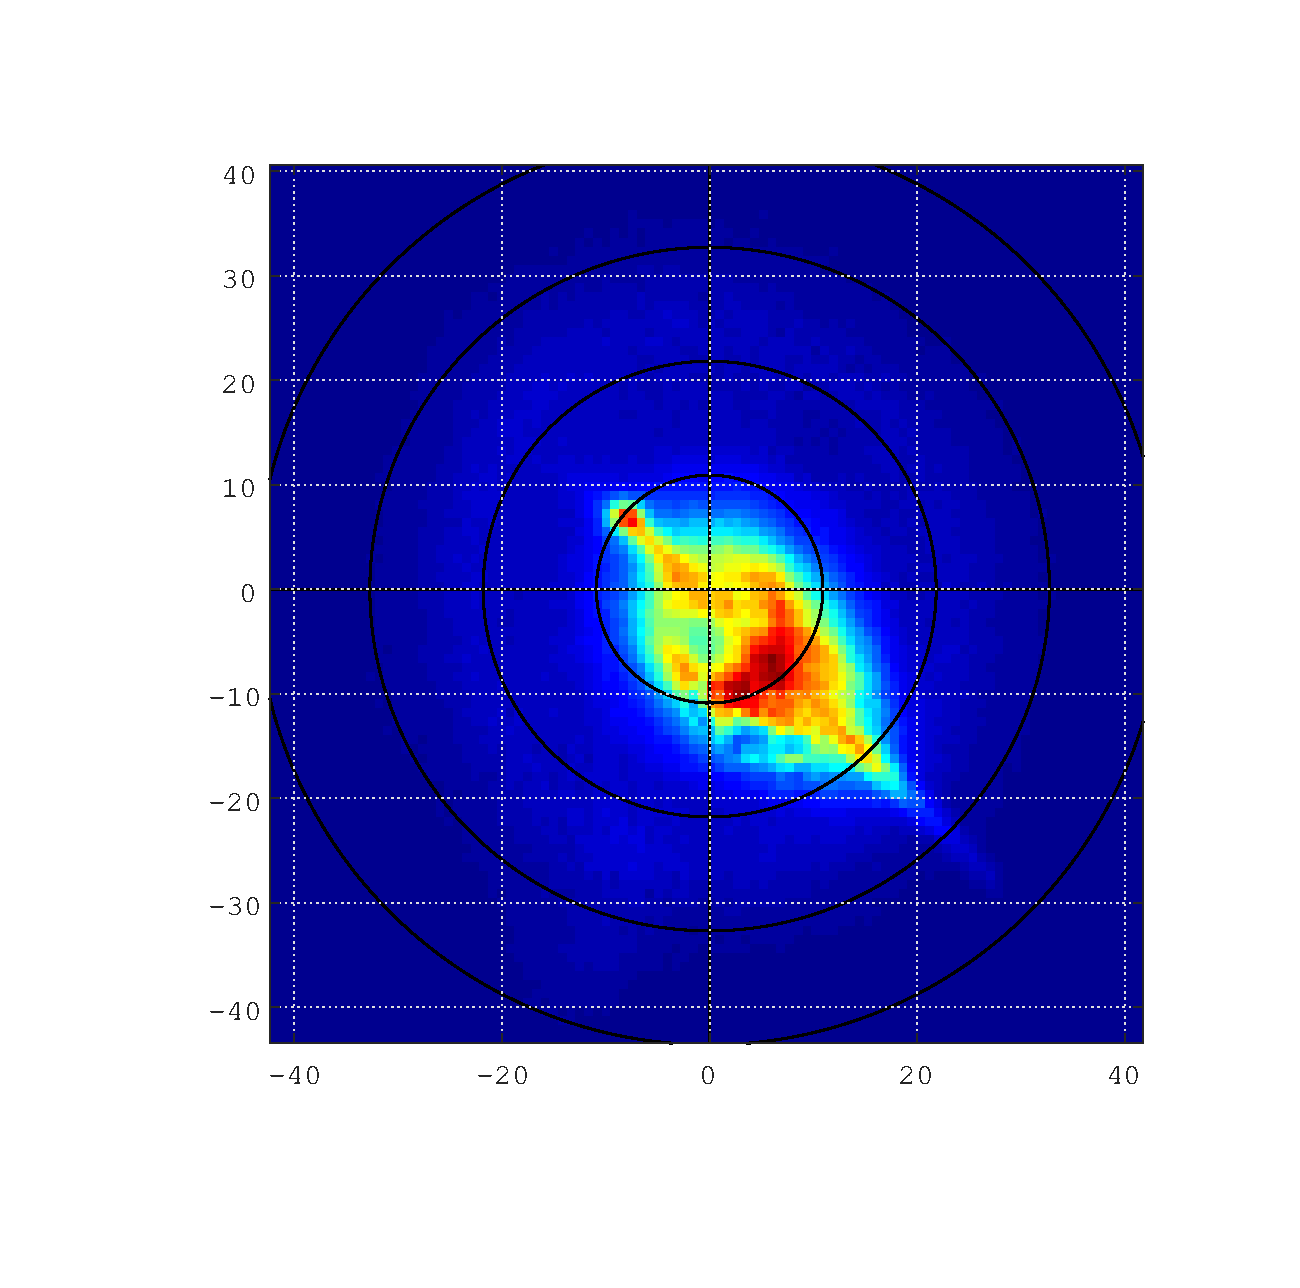
\includegraphics[width=1\textwidth]{Graphics/centre_calibration_after.eps}
  \captionof{figure}{Detector image of all hits after centring. Final values: dX = -0.5 mm, dY = 3mm}
\label{centre_calibration_after}
\end{minipage}
\end{figure}

\paragraph{Metadata parameters used by the detector image translation:}
.\newline
\lstset{language=MATLAB}
\begin{lstlisting}
exp_md.corr.det1.ifdo.dXdY 			= true; % Does this data need detector image translation correction?
exp_md.corr.det1.dX					= -0.5; %[mm] distance the center of detection is displaced left of the origin of the raw image; 
exp_md.corr.det1.dY					= 3; %[mm] distance the center of detection is displaced up the origin of the raw image;
\end{lstlisting}

\subsubsection{detector image rotation}
As seen in Figure \ref{centre_calibration_before}, the detector image shows a line of higher intensity towards the left lower corner of the detector. This is believed to originate from heavier clusters from the molecular beam. The detector image is rotated such, that this line is along the x-axis. 

\begin{figure}[h]
   \centering
    \centerline{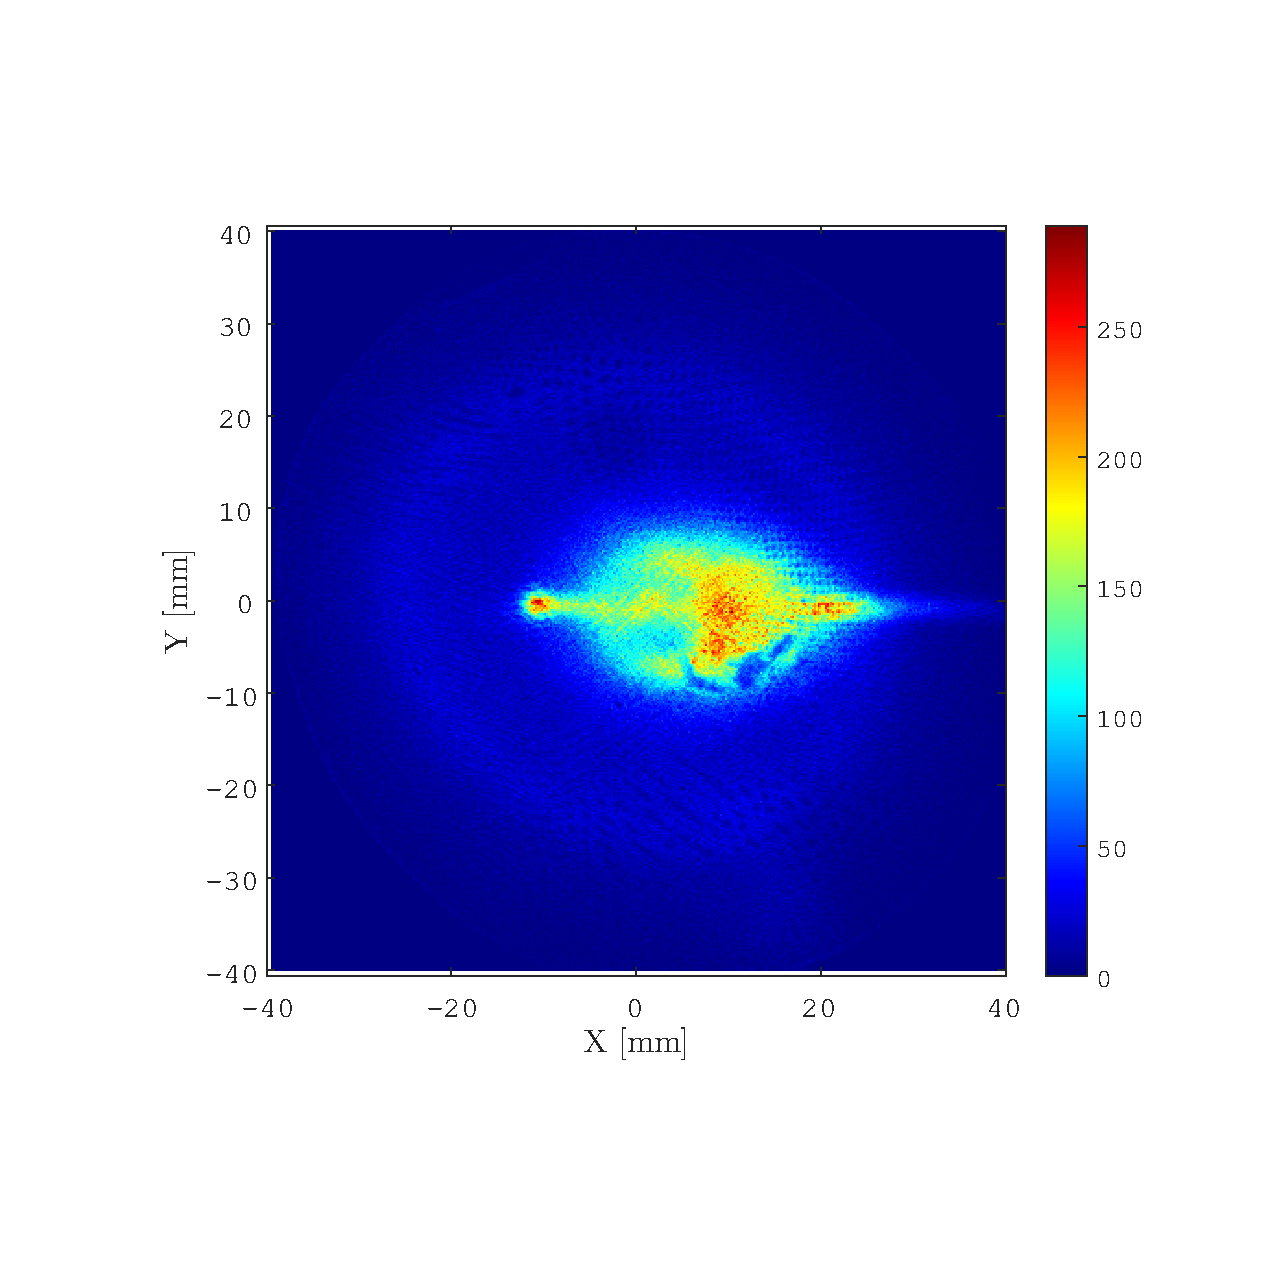
\includegraphics[width=0.5\textwidth]{Graphics/rotation_after.eps}}
\caption{The detector image rotated such that the molecular beam is aligned with the x-axis. In this case, it means an anti-clockwise rotation of 44 degrees.}
\label{Data_structure_schematic}
\end{figure}

\paragraph{Metadata parameters used by the detector image rotation:}
.\newline
\lstset{language=MATLAB}
\begin{lstlisting}
exp_md.corr.det1.ifdo.dTOF  		= true; % Does this data need detector absolute TOF correction?
exp_md.corr.det1.dTheta				= 44;   %[deg] rotation of hits around the raw image centre (anticlockwise);
\end{lstlisting}

\subsubsection{Absolute TOF translation}
The recorded time of flight can have a deviation from the actual one, due to timing differences. These can for instance originate from different signal propagation times of the trigger and the detector signal.

\paragraph{Metadata parameters used by the absolute TOF translation:}
.\newline
\lstset{language=MATLAB}
\begin{lstlisting}
exp_md.corr.det1.ifdo.dTheta 		= true; % Does this data need detector image rotation correction?
exp_md.corr.det1.dTOF 			 	= -16.7; % [ns] The difference between signal propagation times of trigger and hits
\end{lstlisting}

\subsubsection{TOF deviation due to detector-drift tube voltage mismatch}

If the MCP front voltage is not kept at the same voltage as the drift tube, the local field in front of the detector will not be uniform, but curved instead (see Figure \ref{detector_abberation_ray_traces}. This will cause a distortion in the actual TOF, compared to the one predicted assuming a pure drift of the ions in the drift tube. The Time Of Flight will decrease if the detector front is kept at a higher absolute voltage. Moreover, this influence is dependent on the position on the detector. If the ion approaches the detector out of center, the decelleration is later, because the field inhomogenity starts later. Therefore, a correction dependent on radius is needed. First, the correction in TOF is presented, and consequently the correction in splat radius is discussed.

\begin{figure}[h]
   \centering
    \centerline{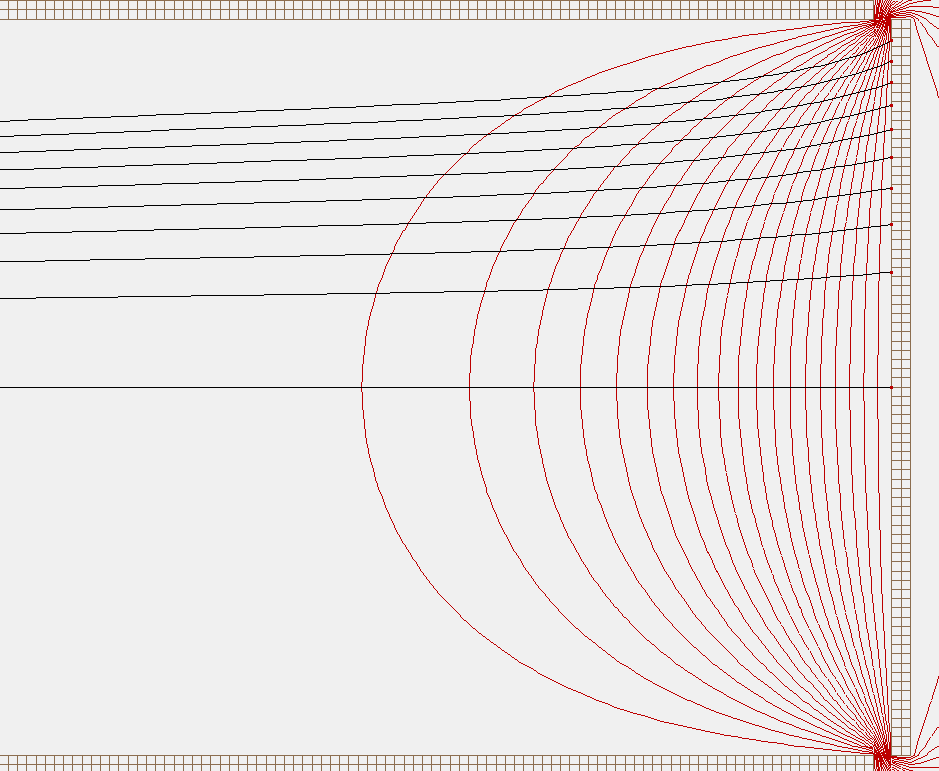
\includegraphics[width=0.5\textwidth]{Graphics/detector_abberation_ray_traces.png}}
\caption{Ray traces showing the non-uniform field around the detector due to the voltage mismatch. In this case, the drift tube is kept at -4 kV and the detector front at -2 kV}
\label{detector_abberation_ray_traces}
\end{figure}


\paragraph{Step 1: Zero kinetic energy TOF correction}

The first step is to adjust the TOF of all particles such that the particles with no kinetic energy (ending up in the centre) have the right time of flight. The correction is done by shifting the measured TOF with an aomunt that is determined from analytical prediction and SIMION simulations. The driving force for the deviation is the difference between the detector and the drift tube voltage. Therefore, we investigate the TOF difference as a function of this difference. We define the following unit-less variables:

\begin{align}
V_{nd} 		= \frac{V_{det} - V_{drift}}{V_{created} - V_{drift}} \\
TOF_{nd} 	= \frac{TOF - TOF_{noKE}}{TOF_{noKE}}
\end{align}
in which $V_{det}$ is the detector front voltage, $V_{drift}$ is the drift tube voltage and $V_{created}$ is the electrostatic potential in which the particle is created. $TOF$ is the measured time of flight and $TOF_{noKE}$ the time of flight of a zero-energy particle, without the lens abberation. This is the variable we are after. Note that if $V_{det} = V_{created}$ ($V_{nd} = 1$), the charge particle has no net gain in energy from source to detector. Therefore, around this voltage configuration the TOF abberation is expected to change considerably. Indeed, a steep asymptote-like behaviour is observed around this point in Figure \ref{dTOF_vs_dV}. 

The variables $V_{nd}$ and $TOF_{nd}$ have a fixed relation, independent of:
\begin{itemize}
\item absolute drift tube voltage
\item mass of particle under study
\item field strength in the source region
\end{itemize}

This relation is approximated by a fitted curve. Since the curve shown in Figure \ref{dTOF_vs_dV} shows behaviour similar to the natural logarithm function, a following polynomial fitting curve is used:

\begin{equation}
TOF_{nd} 	= p_2 \cdot \left(ln(1 -V_{nd}) \right)^2 + p_1 \cdot \left(ln(1 - V_{nd}) \right)
\end{equation}
with $p_i$ the fitting parameters. For the shown example, $p_2 = -1.230e-2$, $p_1 = -1.193e-3$.

\begin{figure}[h]
   \centering
    \centerline{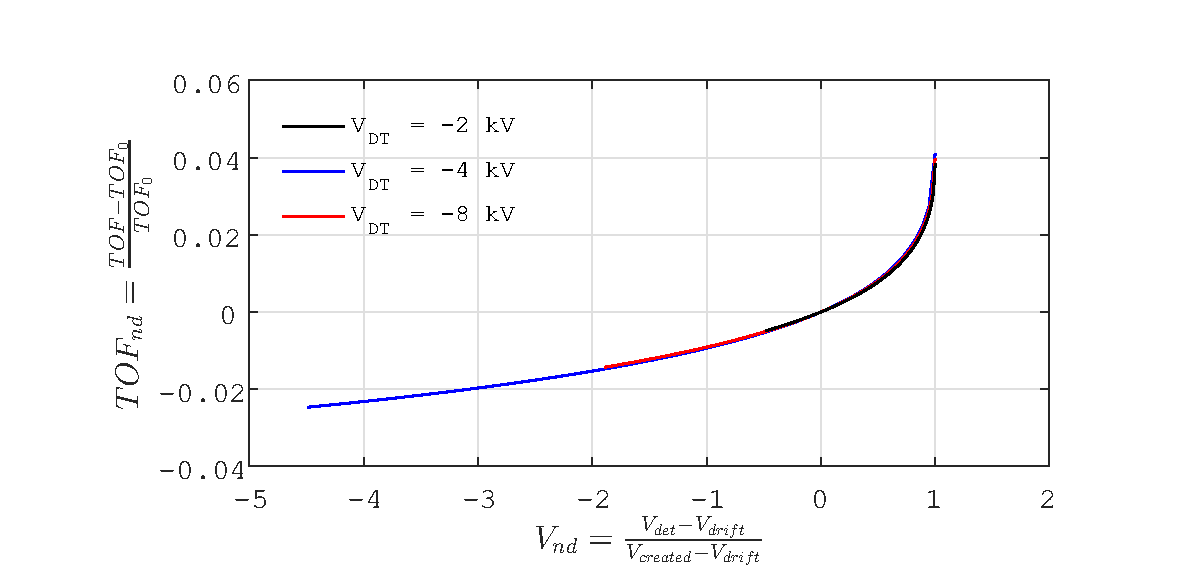
\includegraphics[width=0.9\textwidth]{Graphics/dTOF_vs_dV_dT_-8_-4_-2kV.eps}}
\caption{The Voltage and TOF dimensionless variables plotted for different absolute drift tube voltages. Similar behaviour for varying particle masses, and extraction field strengths.}
\label{dTOF_vs_dV}
\end{figure}

\paragraph{Step 2: TOF correction as a function of radius}
The TOF correction described in step 1 is applied to all hits. However, hits with different splat radii see a different voltage profile along its trajectory, and will therefore be affected differently. We define the following nondimensional variables:

\begin{align}
R_{nd} 		= \frac{R}{R_{det}}\\
TOF_{nd} 	= \frac{TOF_{noKE} - TOF_{corr}}{TOF_{corr}}
\end{align}

in which $R$ is the splat radius, $R_{det}$ the radius of the detector, $TOF_{noKE}$ the corrected time of flight for zero-kinetic energy particles and ${TOF_{corr}}$ the corrected time of flight including the radial correction. This is the variable we are after. The difference in time of flight appears to increase in a quadratic fashion, see Figure \ref{dTOF_dR_nd}. This dependency is, again, independent of absolute voltages, particle masses and interaction field strength. 

\begin{figure}[h]
   \centering
    \centerline{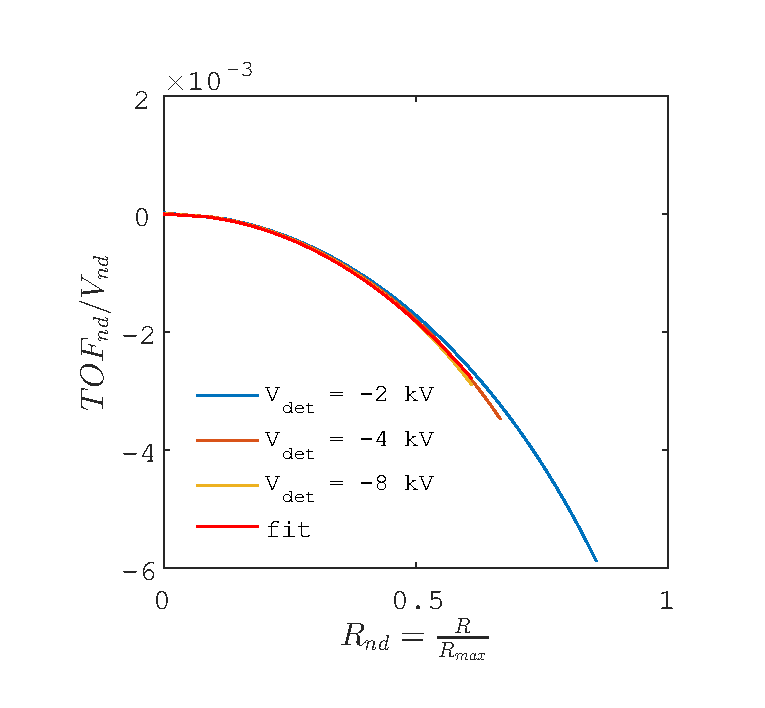
\includegraphics[width=0.9\textwidth]{Graphics/dTOF_dR_nd.eps}}
\caption{The difference in TOF due to a difference in field distortion at different radii. In this example the curve is fitted with $p_2 = -6.32e-3$ and $p_3 = -1.88e-3$. }
\label{dTOF_dR_nd}
\end{figure}

The curve is fitted with the following polynomial:
\begin{equation}
\frac{TOF_{nd}}{V_{nd}} 	= p_2 \cdot \left(R_{nd}) \right)^2 + p_3 \cdot \left(R_{nd}) \right)^3
\end{equation}

The shown correction is validated by comparing it with the theoretical mass to charger conversion factor and the one with and without the correction. The theoretical value is around 965. Without correction, a factor of about 971.7 is found. After correcting, this factor is around 965, so very close to the theoretical value.

\paragraph{Step 3: Correction of splat radius linearity}
Now that the time of flight is corrected for all hits, the splat radius will be corrected. The splat radius is expected to increase linearly with the transverse momentum vector magnitude, and this step corrects the splat radius such that it does. The example trajectories in Figure \ref{detector_abberation_ray_traces} show an outward curve, implicating that the corrected splat radius needs to be smaller than the registered one. This behaviour will be the other way around when the voltage difference is flipped. Therefore, the behaviour is expected to be related to the voltage difference. We assume a inverse proportional relation:

\begin{equation}
\frac{R - R_{corr}}{R_{det}} =  p_1 \cdot V_{nd} \cdot R_{nd}
\end{equation}
in which $R$ is the measured radius and $R_{corr}$ the corrected value. In the example shown in figure \ref{Radius_correction_det_abb}, $p_1 = 0.278$.


\begin{figure}[h]
   \centering
    \centerline{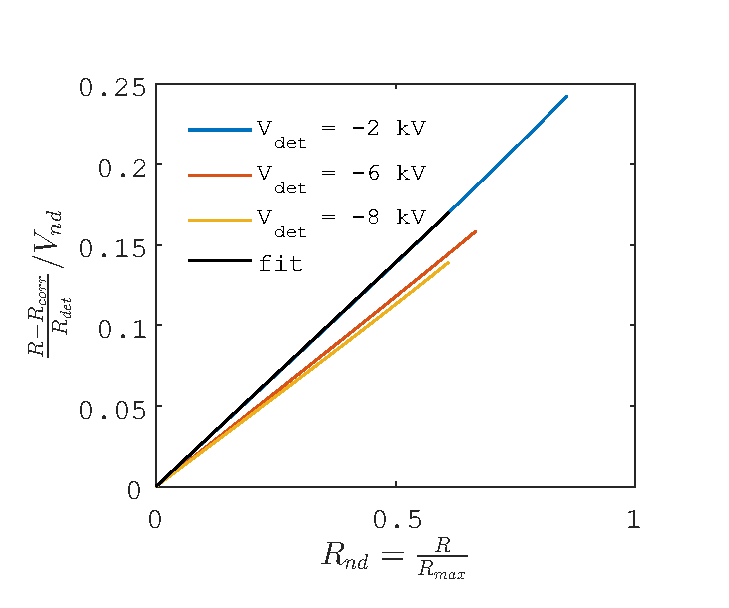
\includegraphics[width=0.6\textwidth]{Graphics/Radius_correction_det_abb.eps}}
\caption{The splat radius correction needed, as a funtion of detector front voltage.}
\label{Radius_correction_det_abb}
\end{figure}

\begin{figure}[h]
   \centering
    \centerline{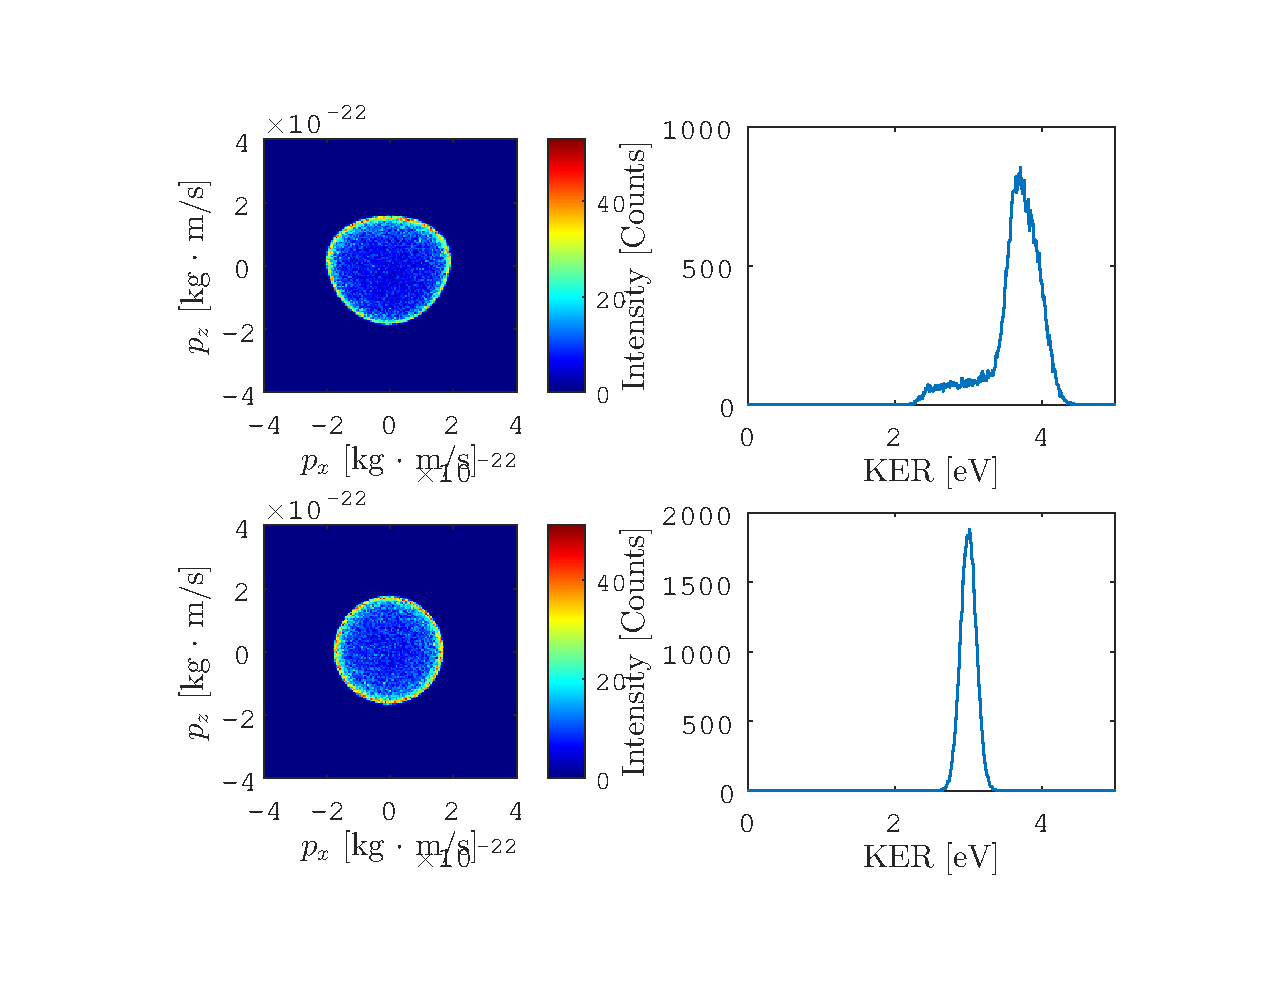
\includegraphics[width=0.8\textwidth]{Graphics/SIMION_det_corr_both.eps}}
\caption{The momenta histograms ($\vec{p_x}$, $\vec{p_z}$) and KER histogram without detector abberation correction (top) and with correction (bottom). SIMION simulations, m = 18 a.m.u, singly charged, KE = 3 eV, $\sigma$(KE) = 0.1eV, 50000 particles. Drift tube @ -4kV, detector front @ -2kV.}
\label{Radius_correction_det_abb}
\end{figure}

\paragraph{Metadata parameters used by the detector abberation correction}
.\newline
\lstset{language=MATLAB}
\begin{lstlisting}
exp_md.corr.det1.ifdo.detectorabb	= true; % Does this data need detector-induced abberation correction?
exp_md.spec.volt			= 0;     %[V] used voltages on electrodes;
exp_md.det.det1.Front_Voltage  	= -2000; % [V] Detector front potential.
exp_md.det.det1.max_radius 		= 40 ; %[mm] Radius of the detector
exp_md.corr.det1.detectorabb.TOF_noKE.p_i	= [-111 -1242 0]*1e-5; % The polynomial fit parameters for the TOF correction, making all zero-kinetic energy TOF's equal to the one without abberation.
exp_md.corr.det1.detectorabb.TOF_R.p_i		= [-1.88  -6.32 0  0]*1e-3;% The polynomial fit parameters for the radial TOF correction
exp_md.corr.det1.detectorabb.dR.p_i			= [0.28 0]% The polynomial fit parameters for the radial correction
\end{lstlisting}

\paragraph{TOF lens abberation correction}
The TOF of a charged particle is not independent of its transversal momentum. In other words; the TOF of a particle with zero kinetic energy is different from the TOF of a particle that has an initial momentum perpendicular to the spectrometer axis. This is a direct consequence of the use of non-uniform fields (lensing). Correcting for this abberation is necessary for the KER determination. We choose a similar approach as presented before, by choosing non-dimensional parameters. Note that this correction is very similar to the one described in `step 1' and '`step 2' of the detector abberation correction.


\paragraph{Step 1: Zero kinetic energy TOF correction}
We define the following dimensionless variables:

\begin{align}
V_{nd} 		= \frac{V_{lens} - V_{drift}}{V_{created} - V_{drift}} \\
TOF_{nd} 	= \frac{TOF - TOF_{noKE}}{TOF_{noKE}} \\
\end{align}
in which $V_{lens}$ is the lens voltage, $V_{drift}$ is the drift tube voltage and $V_{created}$ is the electrostatic potential in which the particle is created. $TOF$ is the measured time of flight and $TOF_{noKE}$ the time of flight of a zero-energy particle, without the lens abberation. This is the variable we are after. 

\begin{figure}[h]
   \centering
    \centerline{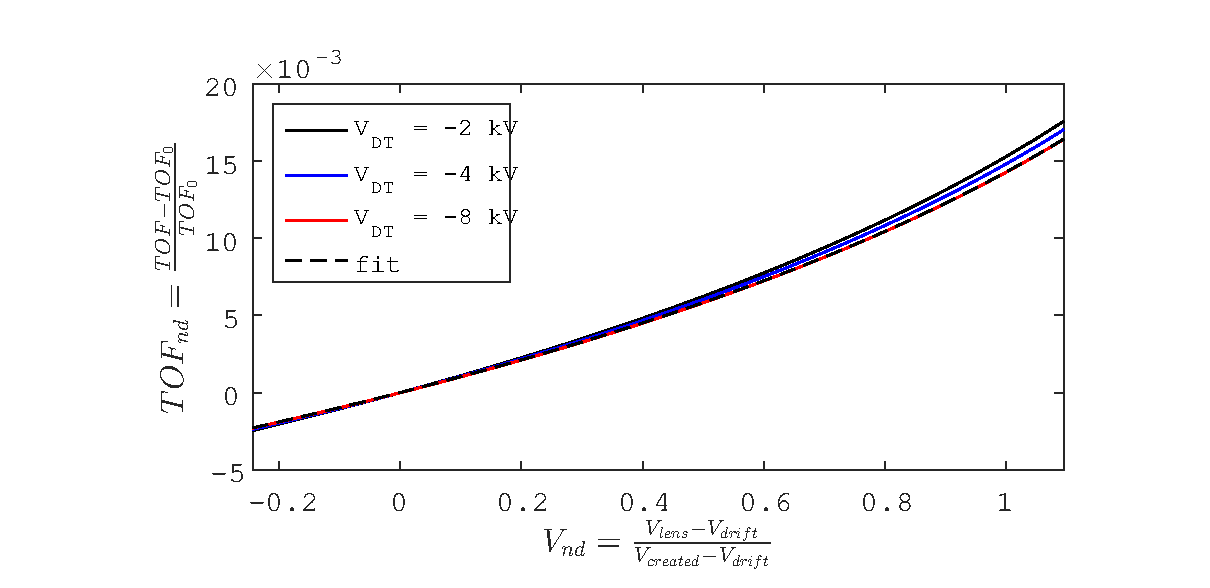
\includegraphics[width=0.8\textwidth]{Graphics/lens_dTOF_vs_dV_dT_-8_-4_-2kV.eps}}
\caption{The Voltage and TOF dimensionless variables plotted for different absolute drift tube voltages. The fit shown uses the parameters $p_3 = 1.13e-3$, $p_2 = 3.48e-3$ $p_4 = 10.4 e-3$}
\label{Radius_correction_det_abb}
\end{figure}

The variables $V_{nd}$ and $TOF_{nd}$ have a fixed relation, independent of:
\begin{itemize}
\item absolute drift tube voltage
\item mass of particle under study
\item field strength in the source region
\end{itemize}

The relation is fitted by a mean-square polynomial fit:
\begin{equation}
TOF_{nd}	= p_3 \cdot \left(V_{nd}) \right)^3 + p_2 \cdot \left(V_{nd}) \right)^2 + p_1 \cdot \left(V_{nd}) \right)^1
\end{equation}

\paragraph{Step 2: TOF correction as a function of radius}
Not implemented yet

\paragraph{Step 3: Correction of splat radius linearity}
The linearity of the radial splat with increasing velocity gets a bit lost with the use of the lens. The following dimensionless variables:

\begin{align}
V_{nd} 		= \frac{V_{lens} - V_{drift}}{V_{created} - V_{drift}} \\
R_{ratio}	= \frac{R_{corr}}{R}
\end{align}

The fit is shown in Figure \ref{dR_correction_fit}.

\begin{figure}[h]
   \centering
    \centerline{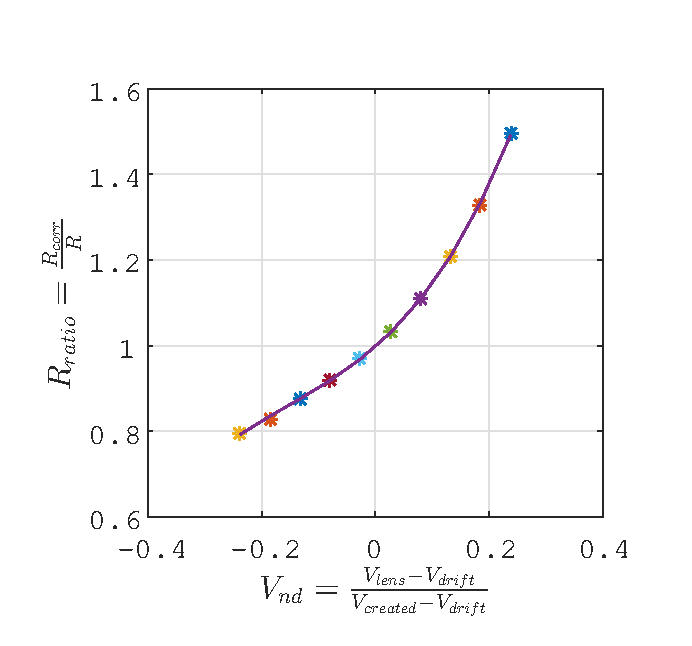
\includegraphics[width=0.8\textwidth]{Graphics/dR_correction_fit.eps}}
\caption{The linearity correction due to the lens abberation.}
\label{dR_correction_fit}
\end{figure}

\begin{figure}[h]
   \centering
    \centerline{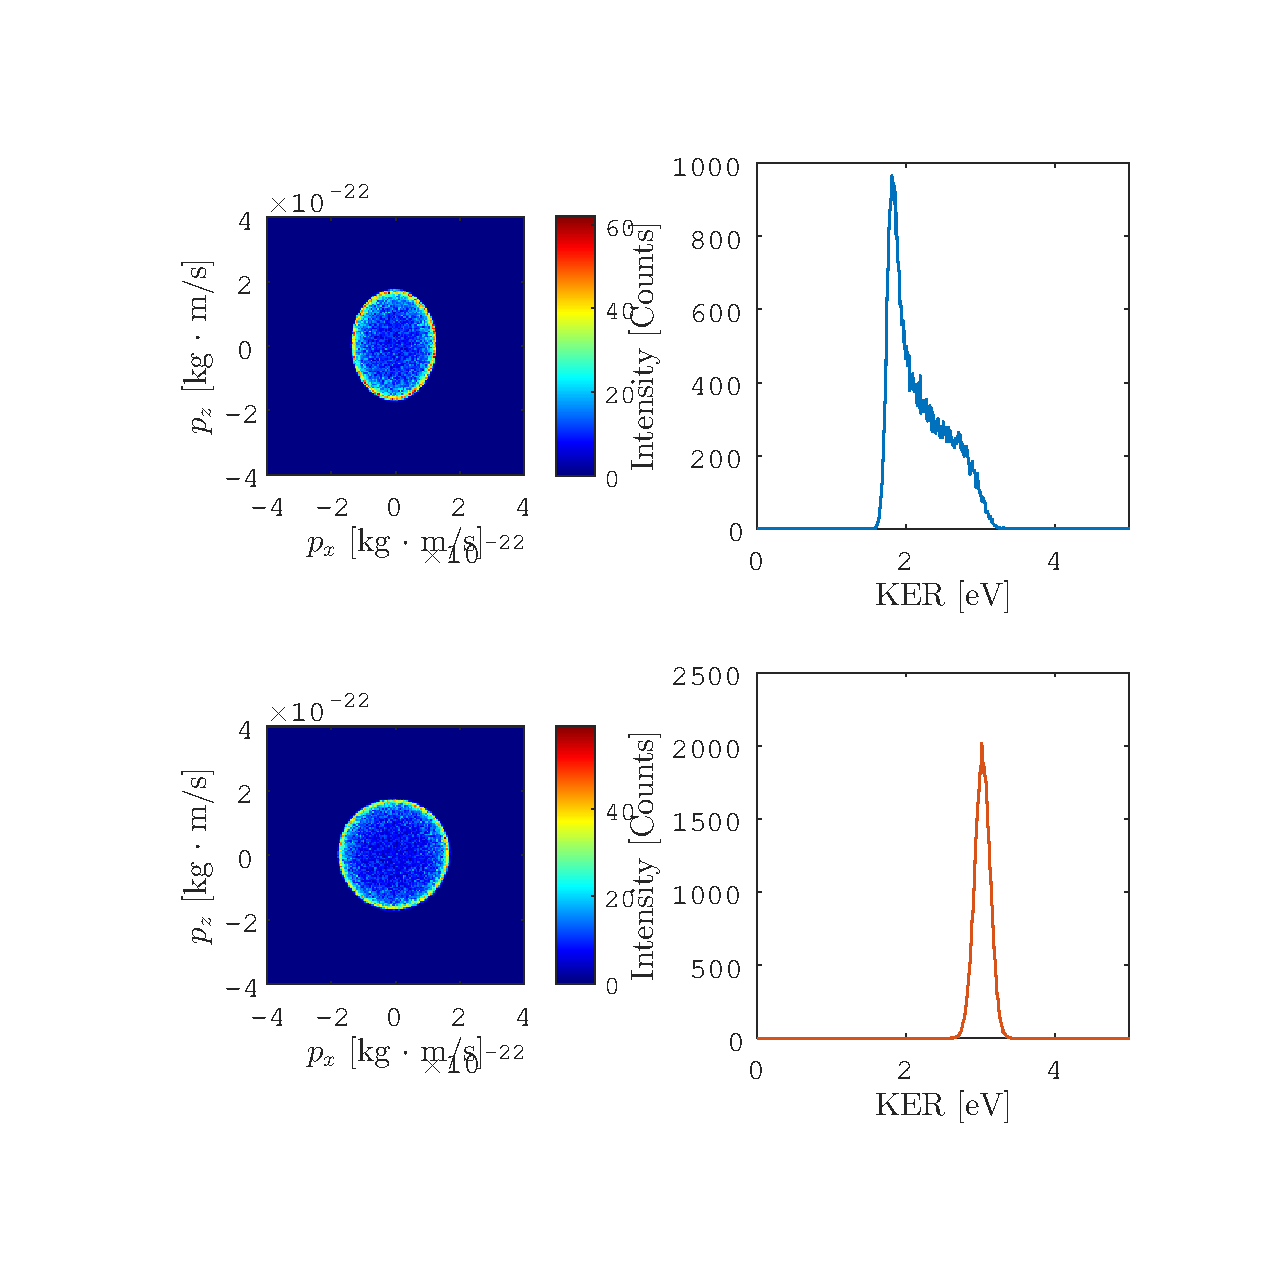
\includegraphics[width=0.8\textwidth]{Graphics/SIMION_lens_corr_both.eps}}
\caption{The momenta histograms ($\vec{p_x}$, $\vec{p_z}$) and KER histogram without lens abberation correction (top) and with correction (bottom). SIMION simulations, m = 18 a.m.u, singly charged, KE = 3 eV, $\sigma$(KE) = 0.1eV, 50000 particles. Drift tube @ -4kV, lens @ -3270V.}
\label{SIMION_lens_corr_both}
\end{figure}

It is tested and verified that the corrections can be applied to the same data, so the detector correction first, followed by the lens abberation correction.

\subsubsection{Non-circular correction}
It can be the case that a spectrometer shows non-circular patterns in the data, where a purely circular pattern is expected from physical principles. There is a routine developed that detects a maximum along the angle in a 2D histogram with the angle (X) and another physical property (Y). 

An example of such a conversion can be found in Figure \ref{R_circle_corr}, the result of a measurement at the EPICEA spectrometer, at the toroidal energy analyzers. The routine calculates a maximum intensity within specified radial regions, called the 'Region Of Interest' (ROI), see the black encircled boxes in Figure \ref{R_circle_corr} left. The maximum-finding procedure uses median filters to the histogram in both angle (phi) and physical quantity (in this case, R) direction, to obtain a maximum line that is smoother and does not get distorted by outliers.

At zero radius, the data points will never be shifted. It is thus important to first calibrate the detection centre correctly. To prevent interpolation out of range, the relative shift at the radial peak value is applied at a radius twice the radial peak value. 

The radial values are shifted in a linear interpolation between the known points from the calibration. The interpolation is thus only applied in radial direction. 

\begin{figure}[h!]
         \centering
    	 \centerline{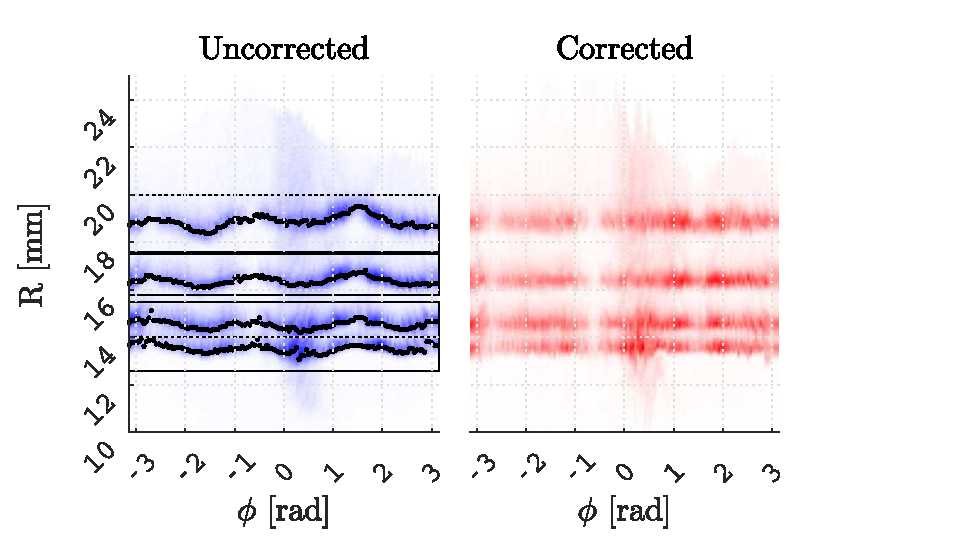
\includegraphics[width=0.8\textwidth]{Graphics/ESCA_R_circle_corr.eps}}
\caption{Left: Histogram showing the angle-dependent electron radial position from a toroidal energy analyzer. In this analyzer, the radial position is converted to electron kinetic energy. The non-circular abberation causes the oscillatory pattern, making the radius to electron energy conversion ambiguous. Right: the corrected electron radial position, showing a horizontal stripe pattern, so that a radial position corresponds to a electron energy. The location of the suspected cause of the instability (physical holders in the spectrometer) are indicated in the right plot. Data: photolines upon C1s ionization of trifluoroacetate (`ESCA molecule') at 411 eV photon energy.}
\label{R_circle_corr}
\end{figure}


